\chapter{The Personal SIP Planner: Implementation}
\label{ch:website}

The end point of the project is a website that applies the Personal SIP rule for one investor, for
the next month. This chapter describes what it does, how it does it, and works through one complete
calculation with real data.

\section{What the user does}

The page is public at \url{https://mainak2929.github.io/personal-sip-planner/}. It needs no login and
no installation.

\begin{table}[H]
\centering
\caption{Inputs and outputs of the planner}
\label{tab:io}
\begin{tabularx}{\textwidth}{@{}XX@{}}
\toprule
The user enters & The user gets \\
\midrule
Risk level: aggressive, moderate or conservative ($\lambda = 2, 4, 8$) & The target split, shown as a bar \\
Monthly SIP amount & How much to buy (or sell) in each fund this month \\
The current value of their three funds & Whether a reset is needed (drift above 5\%) \\
Optionally, last month's return of each fund & Three plain-language lines explaining the split \\
 & The rule's 2020--2025 test result for that risk level \\
\bottomrule
\end{tabularx}
\end{table}

Each month the investor updates the three values from their investment app, optionally adds last
month's returns, and places the purchases shown. Every result is recalculated as soon as an input
changes.

\begin{figure}[H]
\centering
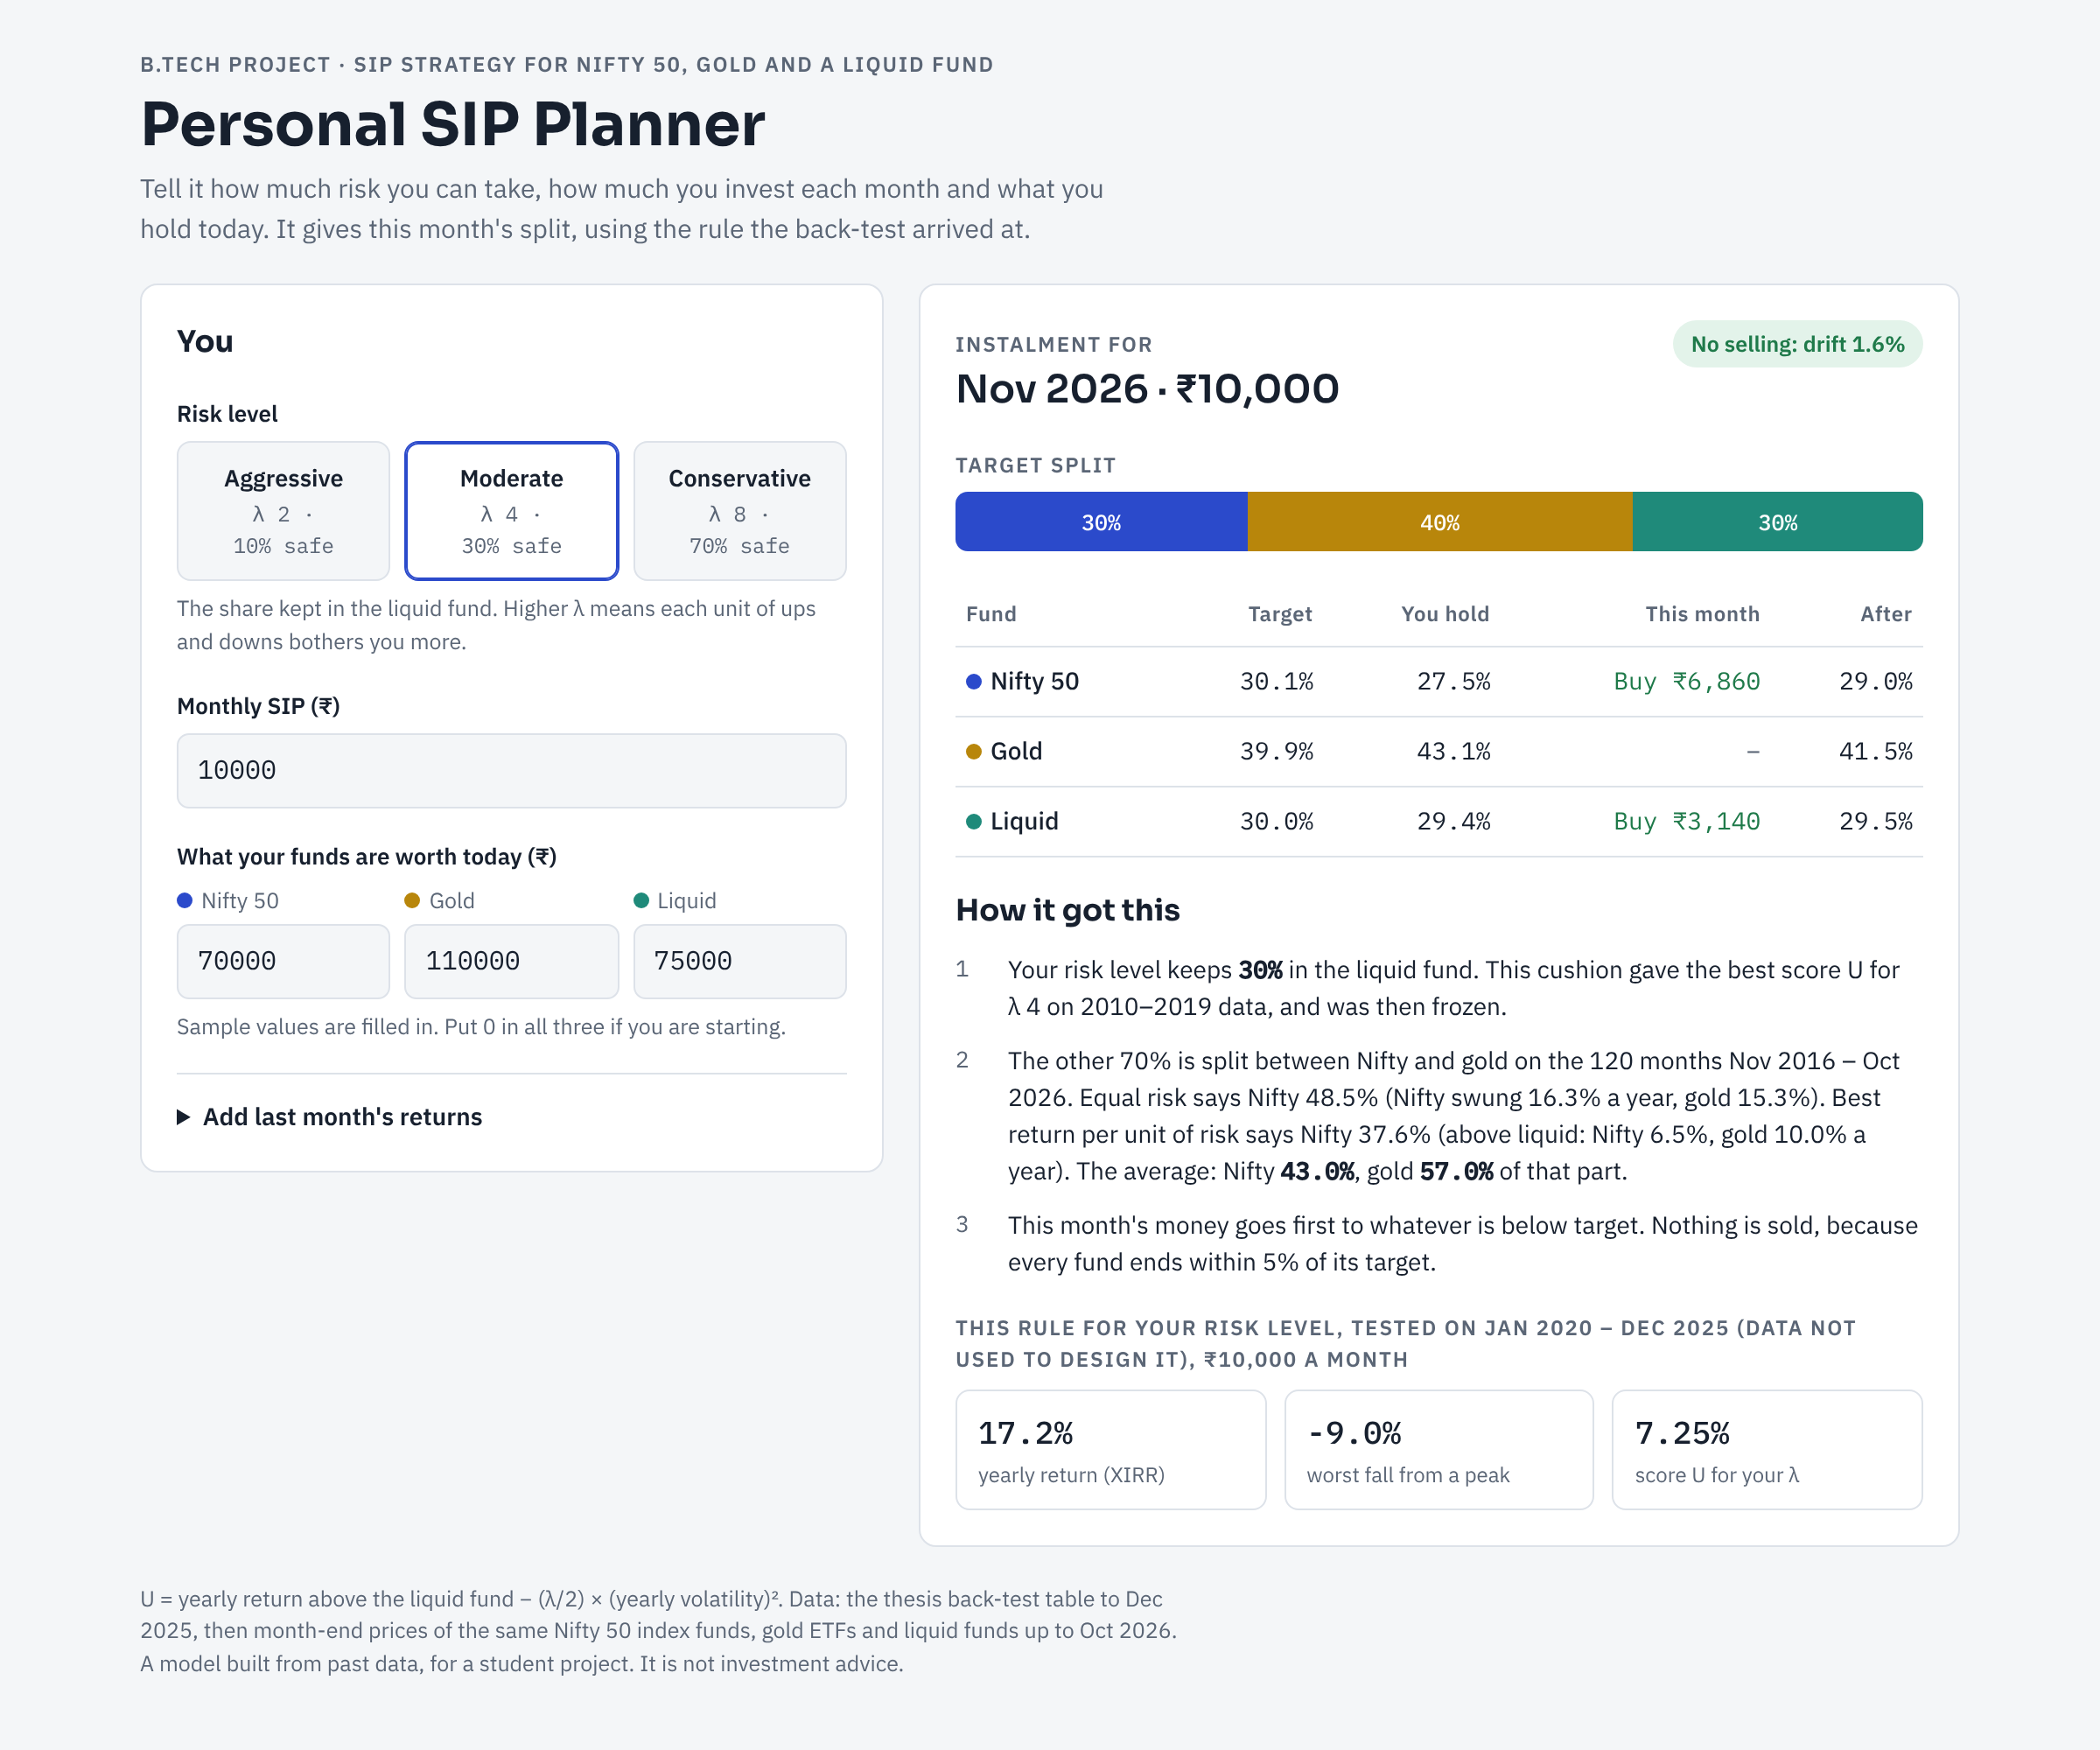
\includegraphics[width=\textwidth]{figures/website.png}
\caption{The planner for a moderate investor planning the November 2026 instalment}
\label{fig:website}
\end{figure}

\section{Design}

\begin{itemize}
  \item \textbf{Runs entirely in the browser.} The page carries the latest 120 months of returns,
        the frozen cushions and the 2020--2025 test results in a small data file (about 6~KB). All
        calculations run on the user's device; nothing the user types is sent anywhere. Months the
        user adds are stored only in their own browser.
  \item \textbf{Same rule as the back-test.} The engine (\code{sip.js}, Appendix~\ref{app:code}) is a
        JavaScript translation of the Python functions used in Chapters~\ref{ch:method}
        and~\ref{ch:results}: \code{optimized\_cash\_buffer} for the target and \code{\_smart\_split}
        with the 5\% band for the purchases.
  \item \textbf{Two-asset closed forms.} With only Nifty and gold in the risky part, risk parity
        uses Eq.~\eqref{eq:rp2} directly, and maximum Sharpe is found by evaluating 2{,}001 evenly
        spaced Nifty shares between the bounds and refining the best one by golden-section search.
  \item \textbf{Hosting.} The site is three static files (\code{index.html}, \code{sip.js},
        \code{data.js}) served free by GitHub Pages from a public repository.
\end{itemize}

\begin{figure}[H]
\centering
\begin{tikzpicture}[
  box/.style={draw, rounded corners, fill=blue!5, align=center, minimum height=8mm, text width=3.4cm, font=\small},
  wide/.style={box, text width=6cm},
  inp/.style={draw, rounded corners, fill=orange!10, align=center, minimum height=8mm, text width=3.1cm, font=\small},
  arr/.style={-{Stealth[length=2.2mm]}, thick}]
\node[inp]  (ret)  at (0,0)      {Last month's returns (optional)};
\node[wide] (s2)   at (0,-1.4)   {2. Window slides: newest month in, oldest out};
\node[wide] (s3)   at (0,-2.8)   {3. Summarise: returns above liquid, volatilities, correlation};
\node[box]  (s4)   at (-2.2,-4.4) {4. Equal risk};
\node[box]  (s5)   at (2.2,-4.4)  {5. Max Sharpe vs liquid};
\node[wide] (s6)   at (0,-6.0)   {6. Average, then add the cushion $\rightarrow$ target};
\node[inp]  (risk) at (-5.6,-6.0) {Risk level $\rightarrow$ cushion};
\node[wide] (s7)   at (0,-7.4)   {7. Fill gaps first; reset only if drift $> 5\%$};
\node[inp]  (hold) at (-5.6,-7.4) {Holdings and amount};
\node[wide] (s8)   at (0,-8.8)   {8. Show split, purchases, reasons};
\draw[arr] (ret) -- (s2); \draw[arr] (s2) -- (s3);
\draw[arr] (s3) -- (s4); \draw[arr] (s3) -- (s5);
\draw[arr] (s4) -- (s6); \draw[arr] (s5) -- (s6);
\draw[arr] (risk) -- (s6); \draw[arr] (s6) -- (s7); \draw[arr] (hold) -- (s7); \draw[arr] (s7) -- (s8);
\end{tikzpicture}
\caption{What the planner computes each time an input changes}
\label{fig:site-flow}
\end{figure}

\section{A complete worked example}
\label{sec:example}

This section follows the exact calculation behind Figure~\ref{fig:website}: a \textbf{moderate}
investor ($\lambda = 4$, cushion $L = 30\%$) on 1 November 2026, investing \Rs10{,}000 and holding
Nifty \Rs70{,}000, gold \Rs1{,}10{,}000 and liquid \Rs75{,}000. The window is the 120 months
November 2016 -- October 2026.

\subsection{Step 1: summarise the window}

\paragraph{Return above liquid.} For each month, the liquid return is subtracted from the Nifty and
gold returns; the 120 differences are averaged and multiplied by 12:
\begin{align*}
  \text{Nifty: }& 0.647872 / 120 = 0.005399 \text{ a month} \times 12 = 6.48\% \text{ a year},\\
  \text{Gold: }& 0.997018 / 120 = 0.008308 \text{ a month} \times 12 = 9.97\% \text{ a year}.
\end{align*}

\paragraph{Volatility.} The squared deviations from the mean are summed, divided by $n-1 = 119$, and
the square root is annualised with $\sqrt{12} = 3.464$:
\begin{align*}
  \text{Nifty: }& \sqrt{0.263199/119} = 4.703\% \text{ a month} \;\Rightarrow\; 16.29\% \text{ a year}
     \quad (V_N = 0.026541),\\
  \text{Gold: }& \sqrt{0.233427/119} = 4.429\% \text{ a month} \;\Rightarrow\; 15.34\% \text{ a year}
     \quad (V_G = 0.023539).
\end{align*}

\paragraph{Co-movement.} The products of the two assets' monthly deviations sum to $-0.0110126$;
divided by 119 and multiplied by 12, the yearly covariance is $C = -0.0011105$, and the correlation
is $-0.044$. Over this decade, Nifty and gold were practically unrelated.

\subsection{Step 2: bounds}

The risky part is $1 - L = 70\%$ of the money. Nifty and gold must each hold at least 10\% and at
most 70\% of the whole portfolio. For \Rs1{,}00{,}000 this means \Rs70{,}000 to split, of which each
must get at least \Rs10{,}000, so the Nifty share of the risky part lies between
$10{,}000/70{,}000 = 14.29\%$ and $60{,}000/70{,}000 = 85.71\%$.

\subsection{Step 3: equal risk}

From Eq.~\eqref{eq:rp2}:
\[
  n_{\text{RP}} = \frac{15.34}{16.29 + 15.34} = \frac{15.34}{31.63} = 48.50\% .
\]
Check with Eq.~\eqref{eq:rc}:
$RC_N = 0.4850\,(0.4850 \times 0.026541 + 0.5150 \times (-0.0011105)) = 0.005966$ and
$RC_G = 0.5150\,(0.5150 \times 0.023539 + 0.4850 \times (-0.0011105)) = 0.005966$.
Both assets contribute equally.

\subsection{Step 4: maximum Sharpe above liquid}

For a Nifty share $w$ of the risky part:
$m = 6.48\%\,w + 9.97\%\,(1-w)$, \;
$v = w^2 V_N + 2w(1-w)C + (1-w)^2 V_G$, \;
score $= m/\sqrt{v}$.

\begin{table}[H]
\centering
\caption{Some of the 2{,}001 mixes evaluated}
\label{tab:ms-search}
\begin{adjustbox}{max width=\textwidth}
\begin{tabular}{@{}rrrr@{}}
\toprule
Nifty share $w$ & Return above liquid $m$ & Volatility $\sqrt{v}$ & Score $m/\sqrt{v}$ \\
\midrule
14.29\% (lowest allowed) & 9.47\% & 13.25\% & 0.715 \\
30.00\% & 8.92\% & 11.60\% & 0.769 \\
\textbf{37.57\%} & \textbf{8.66\%} & \textbf{11.14\%} & \textbf{0.778} \\
50.00\% & 8.22\% & 10.94\% & 0.752 \\
70.00\% & 7.53\% & 12.11\% & 0.622 \\
85.71\% (highest allowed) & 6.98\% & 14.04\% & 0.497 \\
\bottomrule
\end{tabular}
\end{adjustbox}
\end{table}

At the best mix, $w = 0.3757$:
\begin{align*}
  m &= 0.3757 \times 6.48\% + 0.6243 \times 9.97\% = 8.66\%,\\
  v &= \underbrace{0.003746}_{w^2V_N} \; \underbrace{-\,0.000521}_{2w(1-w)C} \; + \underbrace{0.009174}_{(1-w)^2V_G} = 0.012400,
      \qquad \sqrt{v} = 11.14\%,\\
  \text{score} &= 8.66 / 11.14 = 0.778 .
\end{align*}
A 38/62 mix swings 11.1\% a year, less than Nifty (16.3\%) or gold (15.3\%) alone: the
diversification effect of Section~\ref{sec:maxsharpe}.

\subsection{Step 5: the target}

\[
  n = \tfrac12 \times 48.50\% + \tfrac12 \times 37.57\% = 43.03\%,
\]
\begin{align*}
  w_{\text{Nifty}} &= 0.70 \times 43.03\% = 30.12\%, \\
  w_{\text{Gold}} &= 0.70 \times 56.97\% = 39.88\%, \\
  w_{\text{Liquid}} &= 30.00\% .
\end{align*}

\subsection{Step 6: this month's purchases}

The total after investing is $70{,}000 + 1{,}10{,}000 + 75{,}000 + 10{,}000 = \Rs2{,}65{,}000$.

\begin{table}[H]
\centering
\caption{The smart split for the example investor}
\label{tab:example-split}
\begin{adjustbox}{max width=\textwidth}
\begin{tabular}{@{}lrrrrr@{}}
\toprule
Fund & Target & Should hold & Holds now & Gap & Buy \\
\midrule
Nifty & 30.12\% & \Rs79{,}830 & \Rs70{,}000 & \Rs9{,}830 & \Rs6{,}860 \\
Gold & 39.88\% & \Rs1{,}05{,}670 & \Rs1{,}10{,}000 & 0 & 0 \\
Liquid & 30.00\% & \Rs79{,}500 & \Rs75{,}000 & \Rs4{,}500 & \Rs3{,}140 \\
\midrule
Total & & & & \Rs14{,}330 & \Rs10{,}000 \\
\bottomrule
\end{tabular}
\end{adjustbox}
\end{table}

The gaps exceed the instalment, so by Eq.~\eqref{eq:smart} the money is shared in proportion:
$9{,}830/14{,}330 \times 10{,}000 = \Rs6{,}860$ to Nifty and
$4{,}500/14{,}330 \times 10{,}000 = \Rs3{,}140$ to liquid. Afterwards the shares are 29.0\%, 41.5\%
and 29.5\%. The largest drift is gold's 1.6 percentage points, below the 5\% band, so nothing is
sold. These are exactly the figures in Figure~\ref{fig:website}.

\section{Stability of the target}

A natural question is how much one unusual month changes the advice. As a test, an extreme month
was entered for November 2026: Nifty $+1\%$, gold $+20\%$, liquid $+10\%$.

\begin{table}[H]
\centering
\caption{Effect of extreme new months on the moderate investor's target}
\label{tab:stability}
\small
\begin{adjustbox}{max width=\textwidth}
\begin{tabular}{@{}lcccc@{}}
\toprule
Scenario & Equal risk & Max Sharpe & Average & Nifty / Gold / Liquid \\
\midrule
Window to Oct 2026 (as above) & 48.50\% & 37.57\% & 43.03\% & 30.1 / 39.9 / 30 \\
Add Nov: Nifty $+1\%$, gold $+20\%$, liquid $+10\%$ & 50.16\% & 36.45\% & 43.31\% & 30.3 / 39.7 / 30 \\
Add Nov: gold $+60\%$ & 59.68\% & 49.21\% & 54.45\% & 38.1 / 31.9 / 30 \\
Gold $+20\%$ every month for a year & 60.58\% & 30.93\% & 45.76\% & 32.0 / 38.0 / 30 \\
\bottomrule
\end{tabular}
\end{adjustbox}
\end{table}

The 20\% gold month moved the Nifty target by only 0.2 percentage points, for three reasons. It is
one month out of 120. The two advisers react in opposite directions: gold's higher average return
pulls maximum Sharpe towards gold, while gold's higher volatility pushes risk parity away from it.
And the liquid share is the fixed cushion, so the liquid fund's 10\% month cannot change it. Only a
shock large enough to raise gold's volatility sharply (the $+60\%$ case) moves both advisers the
same way. This stability is deliberate: the rule does not chase short-term spikes, which the
estimation-error literature suggests would be costly. The price is that it adapts slowly to a
genuine, lasting change.

\section{Verification}

\begin{itemize}
  \item An automated test runs \code{sip.js} under Node.js on the same 120-month window as the Python
        engine and requires the targets to agree within $10^{-6}$ and the rupee purchases within
        \Rs0.50, for all three profiles. The observed differences were below $10^{-8}$ for the
        targets and \Rs0.003 for the purchases.
  \item A second test checks that the page's data file is exactly the latest 120 months of the
        project's return table.
  \item The page was checked at desktop and phone widths and in light and dark themes.
\end{itemize}

\section{Limitations of the planner}

\begin{itemize}
  \item The risk level is chosen from three fixed profiles rather than measured by a questionnaire.
  \item Taxes and exit loads are not considered when recommending a sale.
  \item The data must be kept current: either the maintainer updates the data file, or the user adds
        each month's returns on the page.
  \item The planner is an educational output of a back-test, not investment advice.
\end{itemize}
